% Für Bindekorrektur als optionales Argument "BCORfaktormitmaßeinheit", dann
% sieht auch Option "twoside" vernünftig aus
% Näheres zu "scrartcl" bzw. "scrreprt" und "scrbook" siehe KOMA-Skript Doku
\documentclass[12pt,a4paper,titlepage,headinclude,bibtotoc]{scrartcl}


%---- Allgemeine Layout Einstellungen ------------------------------------------

% Für Kopf und Fußzeilen, siehe auch KOMA-Skript Doku
\usepackage[komastyle]{scrpage2}
\pagestyle{scrheadings}
\automark[section]{chapter}
\setheadsepline{0.5pt}[\color{black}]


%Einstellungen für Figuren- und Tabellenbeschriftungen
\setkomafont{captionlabel}{\sffamily\bfseries}
\setcapindent{0em}


%---- Weitere Pakete -----------------------------------------------------------
% Die Pakete sind alle in der TeX Live Distribution enthalten. Wichtige Adressen
% www.ctan.org, www.dante.de

% Sprachunterstützung
\usepackage[ngerman]{babel}

% Benutzung von Umlauten direkt im Text
% entweder "latin1" oder "utf8"
\usepackage[utf8]{inputenc}

% Pakete mit Mathesymbolen und zur Beseitigung von Schwächen der Mathe-Umgebung
\usepackage{latexsym,exscale,amssymb,amsmath}

% Weitere Symbole
\usepackage[nointegrals]{wasysym}
\usepackage{eurosym}

% Anderes Literaturverzeichnisformat
%\usepackage[square,sort&compress]{natbib}

% Für Farbe
\usepackage{color}

% Zur Graphikausgabe
%Beipiel: \includegraphics[width=\textwidth]{grafik.png}
\usepackage{graphicx}

% Text umfließt Graphiken und Tabellen
% Beispiel:
% \begin{wrapfigure}[Zeilenanzahl]{"l" oder "r"}{breite}
%   \centering
%   \includegraphics[width=...]{grafik}
%   \caption{Beschriftung} 
%   \label{fig:grafik}
% \end{wrapfigure}
\usepackage{wrapfig}

% Mehrere Abbildungen nebeneinander
% Beispiel:
% \begin{figure}[htb]
%   \centering
%   \subfigure[Beschriftung 1\label{fig:label1}]
%   {\includegraphics[width=0.49\textwidth]{grafik1}}
%   \hfill
%   \subfigure[Beschriftung 2\label{fig:label2}]
%   {\includegraphics[width=0.49\textwidth]{grafik2}}
%   \caption{Beschriftung allgemein}
%   \label{fig:label-gesamt}
% \end{figure}
\usepackage{subfigure}

% Caption neben Abbildung
% Beispiel:
% \sidecaptionvpos{figure}{"c" oder "t" oder "b"}
% \begin{SCfigure}[rel. Breite (normalerweise = 1)][hbt]
%   \centering
%   \includegraphics[width=0.5\textwidth]{grafik.png}
%   \caption{Beschreibung}
%   \label{fig:}
% \end{SCfigure}
\usepackage{sidecap}

% Befehl für "Entspricht"-Zeichen
\newcommand{\corresponds}{\ensuremath{\mathrel{\widehat{=}}}}

%Für chemische Formeln (von www.dante.de)
%% Anpassung an LaTeX(2e) von Bernd Raichle
\makeatletter
\DeclareRobustCommand{\chemical}[1]{%
  {\(\m@th
   \edef\resetfontdimens{\noexpand\)%
       \fontdimen16\textfont2=\the\fontdimen16\textfont2
       \fontdimen17\textfont2=\the\fontdimen17\textfont2\relax}%
   \fontdimen16\textfont2=2.7pt \fontdimen17\textfont2=2.7pt
   \mathrm{#1}%
   \resetfontdimens}}
\makeatother

%Si Einheiten
\usepackage{siunitx}

%c++ Code einbinden
\usepackage{listings}
\lstset{numbers=left, numberstyle=\tiny, numbersep=5pt}

\usepackage{caption}

%Zitate
%\usepackage[round]{natbib}
\usepackage{cite}

%keine Einrückung nach leerzeile
\parindent0pt

%Literaturverzeichnis
\usepackage{babelbib}
\selectbiblanguage{ngerman}

\begin{document}

\begin{titlepage}
\centering
\textsc{\Large Anfängerpraktikum der Fakultät für
  Physik,\\[1.5ex] Universität Göttingen}

\vspace*{4.2cm}

\rule{\textwidth}{1pt}\\[0.5cm]
{\huge \bfseries
  Adiabatenexponent\\[1.5ex]
  Protokoll:}\\[0.5cm]
\rule{\textwidth}{1pt}

\vspace*{3.0cm}

\begin{Large}
\begin{tabular}{ll}
Praktikant:
%	&  Skrollan Detzler\\
 	&  Felix Kurtz\\
% 	&  Michael Lohmann\\
	&  Kevin Lüdemann\\

  E-Mail: 
%	&  skrollan.detzler@stud.uni-goettingen.de\\
	&  felix.kurtz@stud.uni-goettingen.de\\
%	& m.lohmann@stud.uni-goettingen.de\\	
	&  kevin.luedemann@stud.uni-goettingen.de\\

 Betreuer: & Martin Ochmann\\
 Versuchsdatum: & 16.06.2014\\
\end{tabular}
\end{Large}

\vspace*{0.8cm}

\begin{Large}
\fbox{
  \begin{minipage}[t][2.5cm][t]{6cm} 
    Testat:
  \end{minipage}
}
\end{Large}

\end{titlepage}

\tableofcontents

\newpage

\section{Einleitung}
\label{sec:einleitung}
Der Adiabatenexponent ist ein Ausdruck, der durch die Anzahl der Freiheitsgrade eines Gasen bestimmt wird. 
Alternativ kann dieser auch über die spezifische Wärme eines Gases, welche eine Konstante ist, bestimmt werden.
Wir wollen in diesem Versuch auf zwei verschiedene Arten diesen Adiabatenexponenten $\kappa$ bestimmen.
Der erste Versuchsaufbau ist der Aufbau nach Rüchardt und der zweite ist nach Clement-Desormes.

\section{Theorie}
\label{sec:theorie}

\subsection{Ideales Gas}
Als Ideales Gas wird ein Gas bezeichnet, dass als einatomig angesehen wird.
Zum Vereinfachen der Rechnungen wird die Annahme gemacht, dass dieses Gas nur von Punktteilchen gefüllt ist.
Dies vereinfacht die Darstellung von Gesetzen und ermöglicht es die Ideale Gasgleichung auf zu stellen, dessen Produkt von Druck und Volumen nur von der Zahl der Teilchen und deren Temperatur abhängig ist.
\begin{align}
	pV=Nk_BT=nRT\label{eq:ideal}
\end{align}
Hierbei ist die Anzahl der Teilchen N und die Boltzmannkonstante k$_B$ zusammengefasst zu R=N$_A$k$_B$, wobei N$_A$ die Advogardokonstante ist n die Stoffmenge.
\cite[S. 261]{gerthsen}

\subsection{Zustandsänderung in Gasen}
Die Ideale Gasgleichung \eqref{eq:ideal} gilt für ein ideales Gas immer, dennoch kann es sich auf verschiedene Zustandsänderungen verschieden verhalten.
Bei z.B. bleibt der Druck p konstant, so ist das Volumen V proportional zur Temperatur T.
Diese Zustandsänderung wird als Isobar bezeichnet.
Bleibt hingegen das Volumen konstant, so spricht man von einer Isochoren Zustandsänderung.
Die hier interessantere Änderung ist aber die adiabatische Änderung.
Hierbei bleibt die Temperatur konstant und es ändern sich Druck und Volumen, doch das Verhältnis zwischen den beiden bleibt gleich.
Dies ist im allgemeinen sehr schwierig zu realisieren, doch es gibt mittlerweile recht gute Isolierungen, oder der Prozess, der adiabatisch ablaufen soll, wird sehr schnell ausgeführt.

\subsection{Freiheitsgrade}
Die Spezifische Wärme eines Gases ist eine Konstante und aus dieser lässt sich mithilfe der Freiheitsgrade und der Konstanten R, wie oben beschrieben, die Konstante $\kappa$ erstellt.
Die Zusammenhänge ergeben sich aus diesen beiden Formel \cite[S. 262]{gerthsen}
\begin{align}
	c_v=\frac{f}{2}R\\
	c_p=\left(\frac{f}{2}+1\right)R
\end{align}
Teilt man jetzt $c_p$ durch $c_v$, so erhält man den Adiabatenexponenten $\kappa$, welcher durch konstanten festgelegt ist.
\begin{align}
	\kappa=\frac{c_p}{c_v}=\frac{f+2}{f}
\end{align}
Betrachtet man Atome als Punktteilchen, so ist bekannt, das die drei verwendeten Gase CO$_2$, Argon und Luft, welches zu 75\% aus Stickstoff besteht und darüber approximiert wird, die in Tabelle \ref{tab:kappafrei} aufgeführten und die sich daraus ergebenen $\kappa$ Werte besitzen.
\begin{table}[!h]
\centering
\begin{tabular}{|c|c|c|c|}
	\hline
				& CO$_2$	& Argon		& Luft\\
	\hline\hline
	Freiheitsgrade f	& 7		& 3		& 5\\
	$\kappa$		& 1.29		& 1.67		& 1.4\\
	\hline
\end{tabular}
\caption{Freiheitsgrade und $\kappa$ Werte der einzelnen verwendeten Gase}
\label{tab:kappafrei}
\end{table}

\subsection{Adiabatenexponent aus Versuchsaufbau}

\subsubsection{Nach Rüchardt}
Bei dem Versuchsaufbau nach Rüchardt wird ein kleiner Körper in schwingung versetzt und die Periodendauer gemessen.
Aus der Periodendauer T kann anschließend der Adiabatenexponent $\kappa$ bestimmt werden.\\
Der Körper hat eine Masse m, das Rohr eine Querschnittsfläche von A, das Gas den Druck p und es hersche der Luftdruck a, so ergibt sich für die Gleichgewichtslage des Körpers.
\begin{align}
	& mg + a\cdot A = p \cdot A\\
	\Rightarrow & p=a+\frac{mg}{A}
\end{align}
Bewegt sich jetzt der Körper in einer Schwingung um die Strecke $\Delta x$ um die Gleichgewichtslage, so lässt sich die folgende Gleichung für die Bewegung des Körpers auf stellen.
\begin{align}
	m\ddot{x}=A\cdot dp
\end{align}
Dadurch, dass der Prozess adiabatisch erfolgt, gilt pV$^\kappa$=const und es lässt sich nach Differentiation von V die folgende Gleichung aufstellen.
\begin{align}
	& dp=-\kappa p \frac{dV}{V}=-\kappa \frac{pA\Delta x}{V}\\
	\Rightarrow & m \ddot{x}=-\kappa\frac{pA^2\Delta x}{V}
\end{align}
Aus dieser Gleichung folgt jetzt direkt die Gleichung für die Periodendauer T aus der Frequenz $\omega$, die sich durch umstellen der Gleichung nach $m\ddot{x}+\omega^2 \Delta x=\ddot{x} + \frac{\kappa pA^2}{mV}\Delta x$ ergibt.
\begin{align}
	& T = 2\pi\sqrt{\frac{mV}{\kappa pA^2}}
	\Rightarrow & \kappa = \frac{4\pi^2m_\text{eff}V}{A^2pT^2}
\end{align}
Durch umstellen ergibt sich die Formel für $\kappa$.
Hierbei wird die effektive Masse m$_\text{eff}$ verwendet, die auch die Masse des bewegten Gases $m_\text{L}$ mit einberechnet.
\begin{align}
	m_\text{eff} = m + m_\text{L}
\end{align}

\subsubsection{Nach Clement-Desormes}
Aus dem Versuchsaufbau \ref{sec:clem} kann man die 4 Zustände Ablesen.
Zu Begin herscht das normale Volumen V$_0$ des Zylinders mit der Raumtemperatur T$_0$ und dem Druck p$_0$, welcher der Raumdruck b ist.
Nach dem erzeugen des Überdrucks $\Delta$p und dem Temperaturausgleich herscht im Zustand 1 der Druck $p=b+\Delta p_1$.
Durch das Öffnen des Entlastungsventils sinkt der Druck und somit auch die Temperatur in Zustand 2.
Durch den nun folgenden Druckausgleich kommen wir wieder auf das Volumen v$_0$ in Zustand 3.
Nach dem letzten Temperaturausgleich erhalten wir im Zustand 4 eine Druckänderung um $\Delta p_2$.\\
Zustand 1: V=$V_0$, p=b+$\Delta p_1$, T=T$_0$\\
Zustand 2: V=$V_0+\Delta V$, p = b, T=$T_0-\Delta T$\\
ZUstand 3: V=$V_0$, p=b, T=$T_0-\Delta T$\\
Zustand 4: V=$V_0$, p=b+$\Delta p_2$, T=$T_0$\\

Dadurch, dass wir adiabtisch von 1 nach 2 kommen könne wir die Poisson-Gleichung anwenden.
\begin{align}
	(b+\Delta p_1)V_0^\kappa &= b(V_0 + \Delta V)^\kappa\label{eq:vol}\\
	(T_0-\Delta T)(V_0+\Delta V)^{\kappa-1}&=T_0\cdot v_0^{\kappa-1}\label{eq:temp}
\end{align}
Nimmt man jetzt an, dass $\Delta V \ll V_0$, so ergibt sich die unten aufgeführte Gleichung.
\begin{align}
	(V_0+\Delta V)^\kappa=V_0^\kappa\left(1+\frac{\Delta V}{V_0}\right)^\kappa \approx V_0^\kappa+\kappa V_0^{\kappa-1}\cdot \Delta V
\end{align}
So lassen sich jetzt auch die Gleichungen \eqref{eq:vol} und \eqref{eq:temp} wie unten angegeben umformen.
\begin{align}
	\frac{\Delta p_1}{b}&=\kappa\frac{\Delta V}{V_0}\\
	\frac{\Delta T}{T_0}&=(\kappa-1)\frac{\Delta V}{V_0}\\
	\Rightarrow \frac{\Delta T}{T_0}&=\frac{\kappa -1}{\kappa}\cdot\frac{\delta p_1}{b}\label{eq:ges}
\end{align}
Durch den Umstand, dass Zustand 3 in 4 isochor übergeht können wir beide mit der Ideal-Gasgleichung verknüpfen.
\begin{align}
	\frac{b}{b+\Delta p_2}=\frac{T_0-\Delta T}{T_0}=1-\frac{\Delta T}{T_0}
\end{align}
Durch einsetzen von \eqref{eq:ges} und umstellen nach $\kappa$ erhält man die Form, wie sie unten gezeigt ist.
\begin{align}
	\kappa=\frac{\Delta p_1}{\Delta p_1-\Delta p_2}\label{eq:clem}
\end{align}

\section{Durchführung}
\label{sec:durchfuehrung}

\subsection{Adiabatenexponent nach Rüchardt}
\begin{figure}
	\centering
	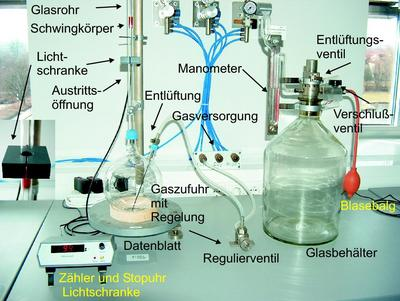
\includegraphics{3725}
	\caption{Bild der beiden Versuchsaufbauten\protect\footnotemark}\label{fig:versuch}
\end{figure}
\footnotetext{Quelle: https://lp.uni-goettingen.de/get/text/3639 29.08.2014 20:08 Uhr}
Der Versuch besteht aus einer Glaskugel, die nach oben hin eine lange dünne Zylindrische Öffnung hat.
Der Aufbau ist in der Graphik \ref{fig:versuch}
zu sehen.
Zum Einlassen des Gases existiert eine Zuleitung, welche über eine Druckkopplungsventil mit drei verschiedenen Gasquellen an der Wand verbunden werden kann.
Am langen Rohr oberhalb der Kugel ist eine Lichtschranke befestigt und es gibt einen kleinen Schlitz unterhalb der Lichtschranke, um das Gas entweichen lassen zu können.
Im Rohr ist ein ebenfalls Zylindrischer Körper, der eng mit der Glaswand des Rohres Abschließt, so dass fast kein Gas vorbei kommt.
Es ist sich mit der ausliegenden Bedienungsanleitung der Lichtschranke vertraut zu machen.\\
Bevor der Versuch gestartet werden kann, muss die Zuleitung mit einem der drei Gasquellen verbunden werden und das Regulierungsventil geöffnet werden.
Damit die Kugel nur noch mit dem gewünschten Gas gefüllt ist, muss die Kugel vor Beginn des Versuches mindestens 3 Minuten mit dem Gas durchgespült werden.
Hierzu wird das Regulierungsventil und das Entlüftungsventil aufgedreht.\\
Ist dieser Vorgang abgeschlossen, so wird das Entlüftungsventil wieder geschlossen und anschließend das Regulierungsventil so eingestellt, dass sich der kleine Zylindrische Körper in einer gleichmäßigen Schwingung um die Lichtschranke befindet.
Es werden jetzt, ohne die Gasregulierung stark zu ändern Messungen von 10 mal einer Schwingung und jeweils 3 mal von 10, 20, 50 und 100 Schwingungen durchgeführt.
Hierzu muss nur die Lichtschranke bedient zu werden.
Dies wird jetzt für die Gase Luft, C0$_2$ und Argon durchgeführt.
Man beginnt jeweils wieder mit dem Durchspülen der Kugel.
Es ist schließlich noch nötig die Masse des kleinen Körpers, der Rohrinnendurchmesser und das Volumen von Kolben und Rohr zu notieren.

\subsection{Adiabatenexponent nach Clement-Desormes}
\label{sec:clem}
Der Versuchsaufbau ist ebenfalls in der Graphik \ref{fig:versuch} von oben zu sehen.
Dieser Aufbau besteht aus einem großen Glaszylinder und einem Manometer.
Zu dem gibt es noch ein Entlüftungs- und Verschlussventil und einen Blasebalg zum erzeugen des Drucks.\\
Zu Beginn des Versuches ist das Verschlussventil zu öffnen und mit dem Blasebalg ein höherer Druck zu erzeugen.
Ist der gewünschte Druck erreicht, so verschließt man das Verschlussventil und führe einen Temperaturausgleich durch.
Für diesen, wird eine Weile lang gewartet, bis sich die Temperatur um Zylinder mit der, der Umwelt ausgeglichen hat.
Anschließend notiert man sich die Höhendifferenz auf dem Manometer.\\
Es werden jetzt je 3 Messungen für verschiedene Öffnungszeiten des Entlüftungsventils gemacht.
Hierzu wird dieses für ca. 0.1s, 1s und 5s geöffnet.
Nach dem kurzen öffnen und schließen ist wieder ein Temperaturausgleich durch zu führen.
Danach wird dann wieder die Höhendifferenz aufgeschrieben.
Es wird wieder, wie oben geschrieben der Druck erhöht und mit der Messreihe fortgefahren, bis alle Messungen durchgeführt sind.
Wichtig ist hierbei stets den Temperaturausgleich zu machen und vor jeder neuen Messung neuen Druck auf zu bauen.

\section{Auswertung}
\label{sec:auswertung}
\subsection{Rüchardt}
In Tabelle \ref{tab:RuechardtWerte} sind die Werte angegeben, die sich auf der Apparatur befanden und diese kennzeichnen: Masse des Schwingkörpers sowie Durchmesser des Rohres und Volumen der Glaskugel.
Außerdem haben wir noch den Luftdruck im Raum gemessen.
Des Weiteren nehmen wir die in der Tabelle angegebenen Werte für die Dichte von Luft und die Erdbeschleunigung an.
\begin{table}[!htb]
	\centering
	\begin{tabular}{|c|c|}
		\hline
		Größe & Wert\\
		\hline
		\hline
		Masse & $m = 8.432~\si{\gram}$\\
		Durchmesser & $d = 11.93~\si{\milli\meter}$\\
		Volumen & $V = 2225~\si{cm^3}$\\
		\hline
		Luftdruck & $b = (1015.7 \pm 0.1)~\si{hPa}$\\ 		
		\hline
		Dichte von Luft & $\rho_L = 1.2~\si{kg/m^3}$\\
		Erdbeschleunigung & $g = 9.81~\si{m/s^2}$\\		
		\hline
	\end{tabular}
	\caption{Den Aufbau kennzeichnende Werte und Konstanten}
	\label{tab:RuechardtWerte}	
\end{table}
In Tabelle \ref{tab:RuechardtAmpl} sind die gemessenen Amplituden des Schwingkörpers für die verschiedenen Gase zu finden.
\begin{table}[!hbt]
	\centering
	\begin{tabular}{|c|c|}
		\hline
		Gas & Amplitude $l$ [cm]\\
		\hline
		\hline
		CO$_2$& $19.5\pm0.5$\\
		Argon & $12.5\pm0.5$\\
		Luft & $17.5\pm0.5$\\
		\hline
	\end{tabular}
	\caption{gemessene Amplitude für die drei verschiedenen Gase}
	\label{tab:RuechardtAmpl}
\end{table}

Mit folgenden Formeln kann man nun über die Masse, welche effektiv schwingt, und den daraus resultierenden Druck $\kappa$ berechnen.
Zur Masse wird noch die Masse der schwingenden Luftsäule addiert.
\begin{align}
	m_{\text{eff}}&= m + \rho_L \cdot A \cdot l\\
	\sigma_{m_\text{eff}}&=\rho_L \cdot A \cdot \sigma_l
\end{align}
Dabei ist $ A = \pi\frac{d^2}{4}$ mit dem Rohrdurchmesser $d$.


Für den resultierenden Druck muss zum Umgebungsdruck noch der von der effektiven Masse erzeugte Druck addiert werden.
\begin{align}
	p &= b + m_{\text{eff}} \cdot \frac{g}{A}\\
	\sigma_p &= \sqrt{\sigma_b^2+\sigma_{m_{\text{eff}}}^2 \cdot \left(\frac{g}{A}\right)^2}\\
	&=\sqrt{\sigma_b^2+\left(\rho_L \cdot g\right)^2 \cdot \sigma_l^2 }
\end{align}

In der Tabelle \ref{tab:RuechardtMasseDruck} findet man die effektiven Massen und Drücke für die verschiedenen Gase, die nach obigen Formeln berechnet wurde.
\begin{table}[!hbt]
	\centering
	\begin{tabular}{|c|c|c|}
		\hline
		Gas & $m_{\text{eff}}$ [g] & $p$ [hPa] \\
		\hline
		\hline
		CO$_2$ & $8.4582 \pm 0.0007$ & $1023.12 \pm 0.10$ \\
		Argon & $8.4488 \pm 0.0007$ & $1023.11 \pm 0.10$ \\
		Luft & $8.4555 \pm 0.0007$ & $1023.12 \pm 0.10$ \\
		\hline
	\end{tabular}
	\caption{Effektive Massen und daraus resultierende Drücke}
	\label{tab:RuechardtMasseDruck}
\end{table}

Mit diesen Wert kann nun $\kappa$ berechnet werden:
\begin{align}
	\kappa&=\frac{64 \cdot m_{\text{eff}}\cdot V }{T^{2} \cdot p \cdot d^{4}}\\
	\sigma_{\kappa}&=\frac{64 ~ V}{T^{3} ~ d^{4} ~ p^{2}} \cdot \sqrt{\left(T ~ m_{\text{eff}}\right)^2 \cdot \sigma_{p}^{2} + \left(T ~ p\right)^2 \cdot \sigma_{m_{\text{eff}}}^{2} + \left(2~m_{\text{eff}}~p\right)^{2} \cdot \sigma_{T}^{2}}
\end{align}

Und aus $\kappa$ folgt die Anzahl der Freiheitsgrade $f$:
\begin{align}
	f&=\frac{2}{\kappa - 1}\\
	\sigma_{f}&=\frac{2 \cdot \sigma_{\kappa}}{\left(\kappa - 1\right)^{2}}
\end{align}

Die Endresultate $\kappa$ und $f$, die mit dieser Messmethode gewonnen wurden, befinden sich in Tabelle \ref{tab:RuechardtKappaF}. 

\begin{table}[!hbt]
	\centering
	\begin{tabular}{|c|c|c|}
		\hline
		Gas & $\kappa$ & $f$\\
		\hline
		\hline		
		CO$_2$ & $1.3037 \pm 0.0005$ & $6.585 \pm 0.011$ \\
		Argon & $1.5944 \pm 0.0010$ & $3.365 \pm 0.006$ \\
		Luft & $1.4051 \pm 0.0008$ & $4.937 \pm 0.009$ \\		
		\hline
	\end{tabular}
	\caption{$\kappa$-Werte und zugehörige Freiheitsgrade der 3 Gase}
	\label{tab:RuechardtKappaF}
\end{table}


\subsection{Clement-Desormes}

\begin{align}
	\kappa&=\frac{\Delta h_{1}}{\Delta h_{1} - \Delta h_{2}}\\
	\sigma_{\kappa}&=\frac{1}{\left(\Delta h_{1} - \Delta h_{2}\right)^{2}} \cdot \sqrt{\Delta h_{1}^{2} \cdot \sigma_{\Delta h_2}^{2} + \Delta h_{2}^{2} \cdot \sigma_{\Delta h_1}^{2}}
\end{align}

\begin{table}[!htb]
	\centering
	\begin{tabular}{|c|c|}
		\hline
		Öffnungszeit [s] & $\kappa$\\
		\hline
		$ 0.1 $ & $ 1.205 \pm 0.022 $ \\
		$ 1.0 $ & $ 1.227 \pm 0.022 $ \\
		$ 5.0 $ & $ 1.177 \pm 0.018 $ \\
		\hline
	\end{tabular}
	\caption{gewichtete Mittelwerte von $\kappa$ \\ für die verschiedenen Öffnungszeiten}
	\label{tab:CDKappa}
\end{table}

\subsection{Mittelwert für $\kappa_\text{Luft}$ aus beiden Messungen}
Betrachtet man beide Messungen, um $\kappa$ von Luft genauer zu bestimmen, ergibt sich folgender gewichteter Mittelwert
\begin{align}
	\kappa_\text{Luft}=1.4042 \pm 0.0008
\end{align}

\section{Diskussion}
\label{sec:diskussion}

\subsection{Rüchardt}
Vergleicht man die Literaturwerte für die Freiheitsgrade und den Adiabatenexponent $\kappa$ der drei verschiedenen Gase aus Tabelle \ref{tab:kappafrei} mit den Messergebnissen aus Tab. \ref{tab:RuechardtKappaF}, fällt auf, dass die Messung sehr genau war und gute Resultate liefert.
So ist die Abweichung bei den $\kappa$-Werten kleiner $5\%$ und die für die Freiheitsgrade kleiner $15\%$.
Die ungenaueste Messung ist die von Argon.
Dabei haben wir zuerst bei den großen Schwingungszahlen angefangen und zum Schluss waren die Einzelschwingungen dran.
Also die umgekehrte Reihenfolge - im Gegensatz zu den beiden anderen Messungen.
Es scheint, dass die zuerst gemachten Messungen ungenauer sind.
Dies wirkt sich dann auf die vermeintlich genauen Messungen mit vielen Schwingungen aus.
All dies kann man bei den Werten aus Tabelle \ref{tab:RuechardtGenauer} im Anhang nachvollziehen.\\
Die Literaturwerte liegen jedoch nicht in den Fehlerintervallen.
Die Fehler wurden also etwas unterschätzt.

\subsection{Clement-Desormes}
Dieser Teilversuch liefert nicht so gute Ergebnisse für $\kappa$ von Luft.
So beträgt die Abweichung zum Literaturwert 1.4 bei allen 3 Messungen etwa $15\%$.
Dies lässt einen systematischen Fehler vermuten.
Eventuell wurde nicht lange genug gewartet, bevor der Temperaturausgleich abgeschlossen war und so das Manometer zu früh abgelesen.

\subsection{Mittelwert für $\kappa_\text{Luft}$ aus beiden Messungen}
Da die Messung nach Rüchardt sehr genau und gut ist, ist auch der Mittelwert aus beiden Messmethoden mit einer Abweichung von $0.3\%$ nah am Literaturwert.
Dieser liegt jedoch nicht im Fehlerintervall.
Wie zuvor schon angemerkt sind die Fehler unterschätzt worden.

\section{Anhang}
\begin{table}[!htb]
	\centering
	\begin{tabular}{|c|c|c|c|}
		\hline
		Gas & Schwingungen & Periodendauer [ms] &$\kappa$\\
		\hline
		\hline
		CO$_2$
		& 1 & $663.9 \pm 1.0$ & $1.319 \pm 0.004$ \\
		& 10 & $666.20 \pm 0.17$ & $1.3094 \pm 0.0007$ \\
		& 20 & $667.7 \pm 0.4$ & $1.3035 \pm 0.0015$ \\
		& 50 & $670.5 \pm 0.4$ & $1.2925 \pm 0.0015$ \\
		& 100 & $672.0 \pm 0.4$ & $1.2870 \pm 0.0014$ \\
		\hline
		Argon
		& 1 & $601.6 \pm 1.0$ & $1.604 \pm 0.005$ \\
		& 10 & $602.80 \pm 0.25$ & $1.5976 \pm 0.0013$ \\
		& 20 & $604.07 \pm 0.31$ & $1.5909 \pm 0.0016$ \\
		& 50 & $606.8 \pm 1.1$ & $1.577 \pm 0.006$ \\
		& 100 & $615.0 \pm 3.1$ & $1.535 \pm 0.016$ \\
		\hline		
		Luft
		& 1 & $639.3 \pm 1.0$ & $1.422 \pm 0.005$ \\
		& 10 & $641.03 \pm 0.29$ & $1.4138 \pm 0.0013$ \\
		& 20 & $642.5 \pm 0.4$ & $1.4073 \pm 0.0016$ \\
		& 50 & $644.5 \pm 0.5$ & $1.3988 \pm 0.0023$ \\
		& 100 & $646.4 \pm 0.4$ & $1.3906 \pm 0.0016$ \\
		\hline
	\end{tabular}
	\caption{Auswertung Rüchardt - alle Messreihen}
	\label{tab:RuechardtGenauer}
\end{table}

\bibliography{literatur}
\bibliographystyle{babalpha}

\end{document}
